% Quick start guide
\documentclass{beamer}
\usetheme {Hannover}
% Title page details
\title{Garbage Collection in JVM}
\subtitle{Tuning}
\author{Miro Kurka}
\institute{Pavol Jozef Safarik University}
\date{\today}
\begin{document}
\begin{frame}
% Print the title page as the first slide
\titlepage
\end{frame}
\begin{frame}{Outline}
    \tableofcontents
\end{frame}
\section{Motivation}

\section{Introduction to Garbage Collection}
\subsection{Memory Overview - Stack and Heap}
\subsection{Objects in memory and How to manage them}
\subsection{Memory Allocation in Java}

\section{Garbage Collection Algorithms in JVM}
    \subsection{Serial garbage collector}
    \subsection{The throughput collector}
    \subsection{CMS}
    \subsection{G1 GC}
    
\section{Tuning - When to choose what}
    \subsection{CMS vs G1 GC}
    \subsubsection{Demo 1 - Docker app}
    \subsubsection{Demo 2 - Low latency server}


\section*{References}

\begin{frame}
    \frametitle{Motivation}
    \begin{itemize}
        \item This seminar is about \texttt{automata} and ML 
        \item Our University basic courses are in Java 
        \item Jobs in KE are usually Java
        \item Interest in low latency programming
        \item Read a paper during undergrad (they lied)
    \end{itemize}
\end{frame}
\begin{frame}

    \frametitle{Introduction to Garbage Collection}
    \begin{columns}
        \column{0.6\textwidth}
        \begin{itemize}
            \item Item 1
            \item You have to manage your memory (\texttt{C,C++})
            \begin{itemize}
                \item Reference counting 
                \item 70\% of bugs\footnote{https://www.chromium.org/Home/chromium-security/memory-safety/}
            \end{itemize}
            \item Brilliant idea 1957 John McCarthy LISP
            \item Item 4
          \end{itemize}
        
        
        \column{0.4\textwidth}
        \begin{figure}
            \centering
            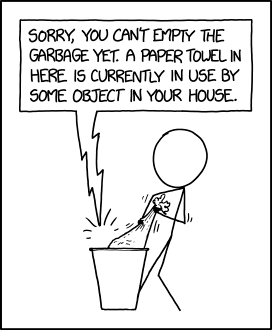
\includegraphics[width=\textwidth]{still_in_use.png}
            \caption[xkcd_1888]{Still in use\footnote{https://xkcd.com/1888/}} % Replace with your image file
        \end{figure}
        
      \end{columns}

\end{frame}
\begin{frame}
    \frametitle{Memory Overview - Stack and Heap}
    \begin{columns}
        \column{0.6\textwidth}
        \begin{itemize}
            \item Item 1
            \item Item 2
            \item Item 3
            \item Item 4
          \end{itemize}
        
        
        \column{0.4\textwidth}
        \begin{figure}
            \centering
            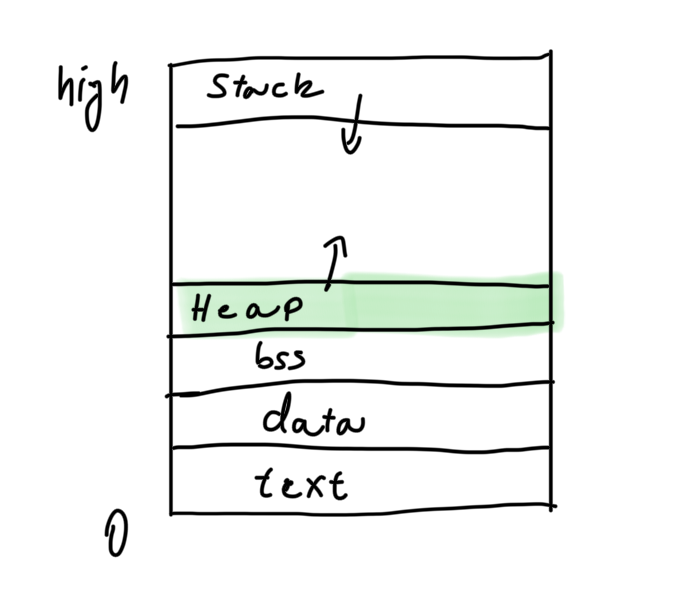
\includegraphics[width=\textwidth]{cmemory.png}
        \end{figure}
        
      \end{columns}
 
\end{frame}



\begin{frame}
    \frametitle{G1 GC}
    \begin{itemize}
        \item default GC since Java 1X\footnote{link}
    \end{itemize}
\end{frame}

\begin{frame}
    \frametitle{References}
    \bibliographystyle{amsalpha}
    \bibliography{jabrefmaster.bib}
\end{frame}

\end{document}